\documentclass{article}

\usepackage{fullpage}
\usepackage{multirow}
\usepackage{float}
\usepackage{booktabs}
\usepackage{tabularx}
\usepackage{hyperref}
\usepackage[normalem]{ulem}
\usepackage[usenames, dvipsnames]{color}
\usepackage{graphicx}
\usepackage{enumitem}
\usepackage{titlesec}
\hypersetup{
    colorlinks,
    citecolor=black,
    filecolor=black,
    linkcolor=red,
    urlcolor=blue
}

\title{SE 3XA3: Development Plan\\Title of Project}

\author{Team 28, Tuples1
		\\ Suhavi Sandhu, sandhs11
		\\ Shabana Dhayanath, dhayanas
		\\ Joseph Lu, luy89
}

\date{\today}

\begin{document}

\maketitle

\newpage

\pagenumbering{roman}
\tableofcontents
\listoftables
\listoffigures

\begin{table}[bp]
\caption{\bf Revision History} \label{TblRevisionHistory}
\begin{tabularx}{\textwidth}{p{3cm}p{2cm}X}
\toprule {\bf Date} & {\bf Version} & {\bf Notes}\\
\midrule
2017-09-29 & 0.0 & Initialization\\
2017-12-06 & 1.0 & Revision 1\\
\bottomrule
\end{tabularx}
\end{table}



\newpage

\pagenumbering{arabic}

Development Plan of our product Password Protection Program.

\section{Team Meeting Plan}
The team will be meeting \sout{twice} \textcolor{blue}{once a week, every week outside of labs, on Fridays} at Thode library. \sout{We have decided to rotate the roles every other week to split responsibilities equally.}\\\\
\textbf{Shabana} - Researcher, Encryption\\
\textbf{Suhavi} - Team Leader, GUI\\
\textbf{Joseph} - Scribe, Database\\

% Table goes here

\begin{table}[bp]
\caption{\bf Meeting Minutes Template} \label{TblMeetMin}
\begin{tabularx}{\textwidth}{ |X||X||X||X| }
    \hline
    \hline
        \multicolumn{4}{|c|}{\textbf{Meeting Minutes}} \\ 
    \hline
    \hline

    \textbf{Meeting no} & \textbf{Location} & \textbf{Meeting Date} & \textbf{Attendees}\\
    \hline
	
	 & & & \\

    \hline

    \multicolumn{4}{|l|}{\textbf{Update on what happened since last meeting: }} \\
		
    \multicolumn{4}{|l|}{ }\\
    \multicolumn{4}{|l|}{ }\\

    \hline
    
    \multicolumn{4}{|l|}{\textbf{Issues discussed this meeting: }}\\

    \multicolumn{4}{|l|}{ }\\
    \multicolumn{4}{|l|}{ }\\ 

    \hline

    \multicolumn{4}{|l|}{\textbf{What to do until next meeting: }} \\

    \multicolumn{4}{|l|}{ }\\
    \multicolumn{4}{|l|}{ }\\

    \hline
        \multicolumn{4}{|l|}{\textbf{Decisions made: }} \\
    \hline
\end{tabularx}
\end{table}


The meeting agenda will be filled out by the scribe after every meeting and uploaded to the git repository for all members to access. Below is a template for the meeting minutes. It notes down the details of the meeting and also provides a guideline for the meeting’s progression. Ideally, we will start by updating the rest of the team with what we have accomplished since the last meeting, followed by items that need to be addressed (problems, opinions, questions), and at the end, what needs to be done by the next meeting. There will also be a written statement on decisions made during the meeting. \hyperref[TblMeetMin]{Meeting Minutes Template}


\section{Team Communication Plan}

The team will primarily use the phone to communicate any issues, changes and progress made on the project. For minor announcements, there will be a Facebook group where we can schedule and confirm meeting times. If there is an important issue that has to do with the code or design of the project, we will be using git issues. When working on the reports, we will be using Google Docs to allow everyone to contribute at the same time and then the scribe will format them into latex for uploading.

\newpage

\section{Team Member Roles}

\textbf{Team Leader} - Schedules meetings and delegates work to the other members as well as him/herself. Ideally, this member will make sure the git repo has no conflicts and looks clean.\\\\
\textbf{Scribe} - Will be in charge of writing meeting minutes as well as writing reports using Latex. This person ideally has experience using Latex.\\\\
\textbf{Researcher} - Will actively learn about the technology we will be implementing in our project. In our case, this will heavily focus on cryptography and documentation from the original product.\\\\
\textbf{Programmer} - All team members will play the role of the programmer as there will be a lot to code.

\section{Git Workflow Plan}

\textbf{Branching Workflow}
\begin{itemize}
    \item \sout{master - branch to host our stable code}
    \item \sout{develop - branch to develop our program}
    \item each \sout{additional} branch is used to implement specific parts of the program
\end{itemize}
Tags will be use when major milestones are reached or there is a major issue that needs attention.\\
Milestones will be used to divide our workload and allow the users to work in parallel.

\section{Proof of Concept Demonstration Plan}
\subsection{Will implementation be difficult?}
The hardest part of the program for us to implement is probably going to be integrating the database into our Python GUI program as our developers have not formally programed in \sout{MySQL} \textcolor{blue}{SQLite}. As we are currently taking a databases course, we will take advantage of those resources and ask the teaching assistants and instructor for clarification when needed.
\subsection{Will testing be difficult?}
\sout{Testing the encryption on our program may be difficult as we are not hackers and do not really have experience or knowledge in trying to break through encryptions.} \textcolor{blue}{The testing of the Python cryptography library that we will be using for the project is out of our scope as we do not have the necessary knowledge or techniques to do so. Instead, we will be assuming that as it is a Python library, Python has conducted sufficient testing to ensure the security of the library.} Therefore, we will mainly focus on testing the user interface. \sout{We will also be researching the Python cryptography library that we intend to use to ensure its credibility.}
\subsection{Is a required library difficult to install?}
The required libraries should be easy to install with the python package manager pip. \textcolor{blue}{The libraries that will need to be installed for the project are cryptography, peewee, pyperclip and tkinter.}
\subsection{Will portability be a concern?}
Portability should not be a concern as long as all the dependencies are downloaded.

\section{Technology}
We will be using Python as the main language to create our application. Our main library to create the GUI is the Python library tkinter. The encryption method we will use is provided by the python library cryptography. The primary IDE we will use is IDLE and the primary form of testing will be done on pyunit. Our documentation generation will be done with Doxygen and our reports will be written in latex. The database that will store the usernames and passwords will be \sout{MariaDB} \textcolor{blue}{SQLite via peewee}.

\section{Coding Style}
We are planning to following the Python coding style\\
\href{https://google.github.io/styleguide/pyguide.html}{Python Coding Syle}

\section{Project Schedule}
\href{run:../../ProjectSchedule/Gantt-FinalSubmission.pdf}{Gantt chart}

\begin{figure}[h]
	\centering
	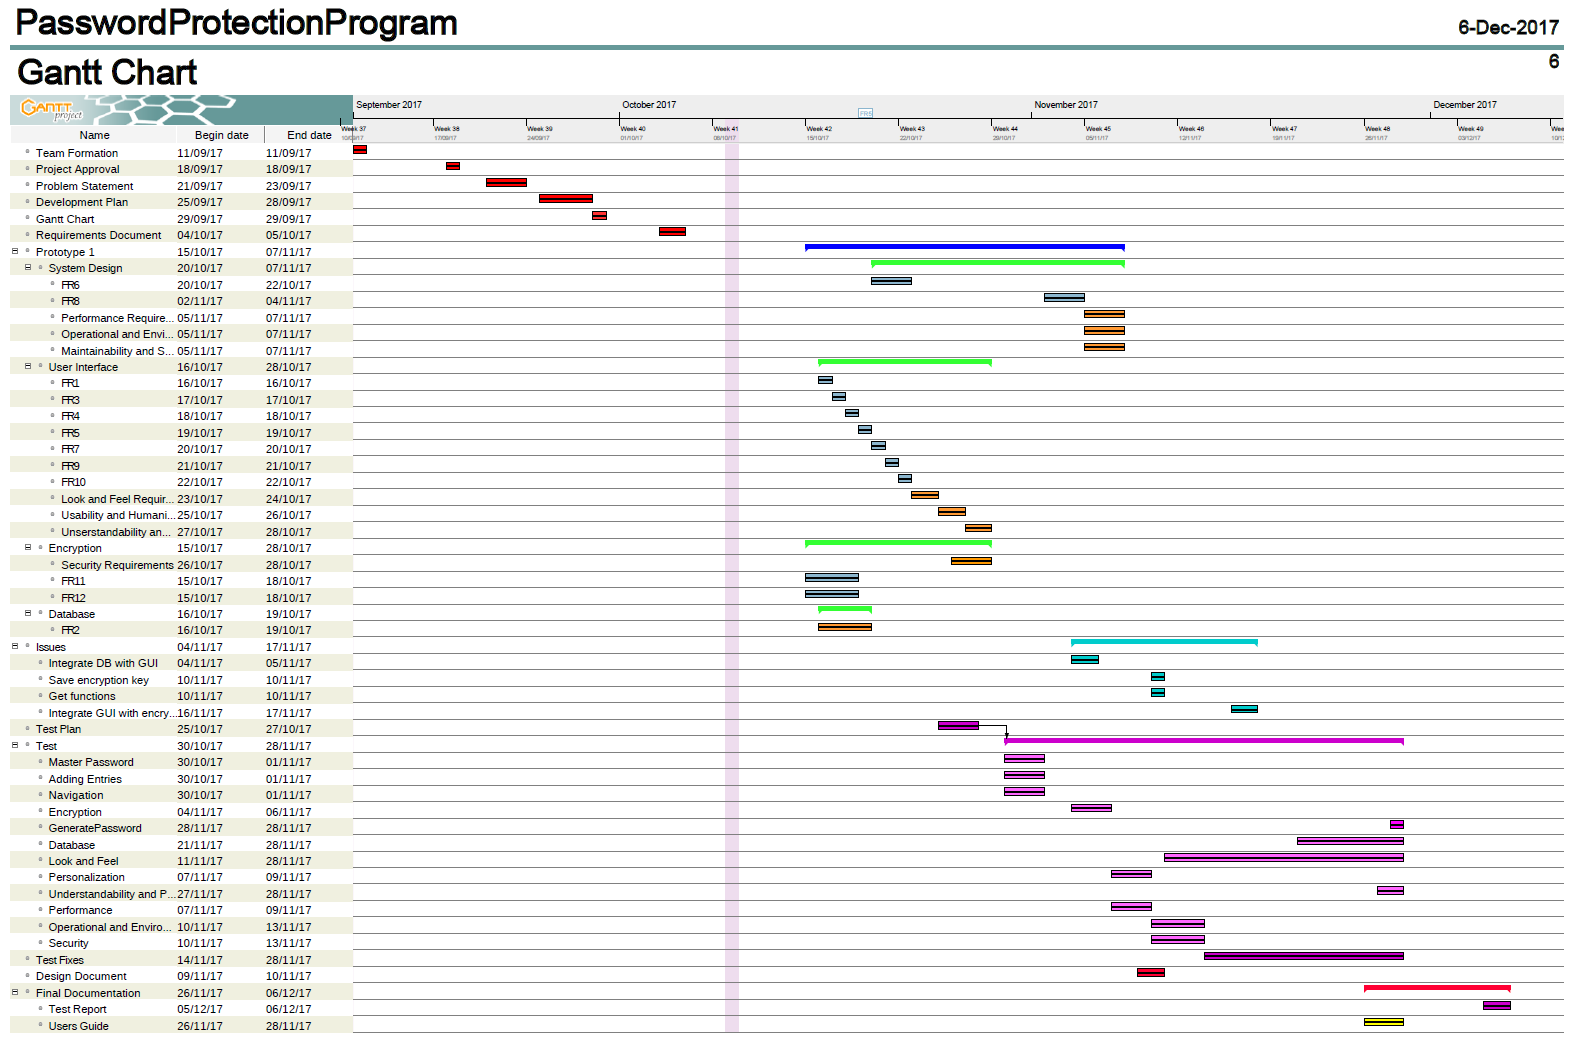
\includegraphics[scale=0.6]{images/Gantt.png}
	\caption{Gantt Chart}
	\label{fig:gantt}
\end{figure}

\section{Project Review}
\textcolor{blue}{When looking back on the development plan after finishing the project, we see that we may have been a bit ambitious in the organization of roles and work. Although we had initially intended to rotate the member roles every week, we were quick to realize that this wasn't really feasible and hard to keep track of in the long run. Therefore, the major roles were left as initially assigned throughout the project.} \\

\textcolor{blue}{Also, we had hoped to have 2 meetings a week, we could rarely get a significant amout of work done during the lab periods so instead we often met of Fridays so that we could work on a large portion of the project at once.} \\

\textcolor{blue}{The team communicated with each other as intended and used separate git workflow branches for the different parts of the code which really facilitated staying on track with the implementation even though we were all working on separate parts.}

\end{document}
